\section{Evaluation}
\label{sec:evaluation}

We ask six questions. \textbf{Q1} quantifies the deployability trade-off
against same-stack baselines. \textbf{Q2} isolates PIECEWISE Graph execution
from the fixed-slot mechanism. \textbf{Q3} measures capacity-bounded waves
against graph-compatible full-layer staging. \textbf{Q4} isolates
transfer--compute overlap. \textbf{Q5} tests sensitivity to slot capacity and
bounded request overlap. \textbf{Q6} evaluates model-contract generality and
accounts for resources and unsupported boundaries.

\subsection{Experimental Methodology}

\paragraph{Platform and software.}
Experiments use one Ascend 910B2 with 65,536~MiB HBM and tensor parallelism
one, hosted by a 192-core Kunpeng-920 server with 2.0~TiB DRAM. Models use BF16
weights. The managed stack pins PyTorch 2.10.0, torch-npu 2.10.0.post2, vLLM
commit \texttt{ad7125a}, and vLLM-Ascend commit \texttt{4806367}. Each run
manifest records the complete command, model and dataset digests, source-tree
digest, environment, device, graph mode, and service-release custody.

\paragraph{Workloads and controls.}
The cost-anchor, overlap, and capacity campaigns use a frozen 64-request
prefill-heavy ShareGPT bucket with
\FormalPromptMin--\FormalPromptMax prompt tokens (median
\FormalPromptMedian), generate 32 tokens at temperature zero and seed 42,
disable prefix caching, and set both concurrency controls to one. The
full-layer/multi-wave campaign uses a
separate frozen 200-request ShareGPT manifest and 128 output tokens. Every
formal unit starts a fresh service. Counterordered comparisons use three start
pairs; the paired estimator is the exponential of the mean, across starts, of
the median per-request log latency ratio. We report a 10,000-replicate
hierarchical bootstrap with seed 20260823: 95\% intervals for TTFT effects and
90\% intervals for the preregistered TPOT equivalence test (margin $\pm5\%$).
For the Qwen3 performance campaigns, the 14-GiB AutoConfig manages 12 of the
model's 48 MoE layers (one layer in each four-layer group); all four baseline
arms and Q3--Q5 use this identical layer selection. Q6 is a separate
capability qualification and exercises the model-specific layer counts shown
in Table~\ref{tab:qualification}.

The c1 Graph qualification uses the frozen standard-v1 ShareGPT, HumanEval,
and GSM8K buckets (200, 164, and 200 requests), generates
four tokens, and holds the same Qwen3 model, 64 slots, 14-GiB host target,
2-GiB KV cache, request order, and sampling controls across Eager and PIECEWISE
Graph modes. Both concurrency controls are one; each bucket uses three
counterordered fresh-start pairs. LongBench is retained separately as an
adverse boundary because all 200 frozen requests exceed the current
8,192-token context configuration.

\paragraph{Baseline roles.}
Full-resident vLLM-Ascend is the HBM and latency cost anchor, not a
memory-matched competitor. Native weight prefetch and legacy layered offload
are same-stack deployment competitors, admitted to performance comparison only
if they pass exact-token parity. \texttt{Slot+Eager} is the matched causal
control for Graph execution: it retains the same slot bank, host store, wave
plan, and lifecycle protocol as \texttt{Slot+PIECEWISE}. Full-layer staging
is the matched design alternative to the complete bounded-wave path. Because
overflow also selects the eager wave executor, Q3 is not a one-factor isolation
of partitioning alone. Serial staging is the one-factor ablation for overlap.

\paragraph{Fail-closed gates.}
A reportable unit must complete all requests, match complete output-token
arrays by request ID, retain fixed slot and map addresses, publish no stale
transfer, violate no owner/version lease, avoid NPU/ACL errors, emit a release
acknowledgment, and retain raw artifacts. Graph arms must additionally capture
and replay every graph-designated PIECEWISE ACLGraph component without
unintended fallback; the explicitly selected eager overflow path is part of the
execution contract and is not counted as fallback. Eager controls must record
Graph as disabled. A completed arm that fails exact-token comparison is
retained but excluded from latency comparison.

\begin{figure*}[!t]
  \centering
  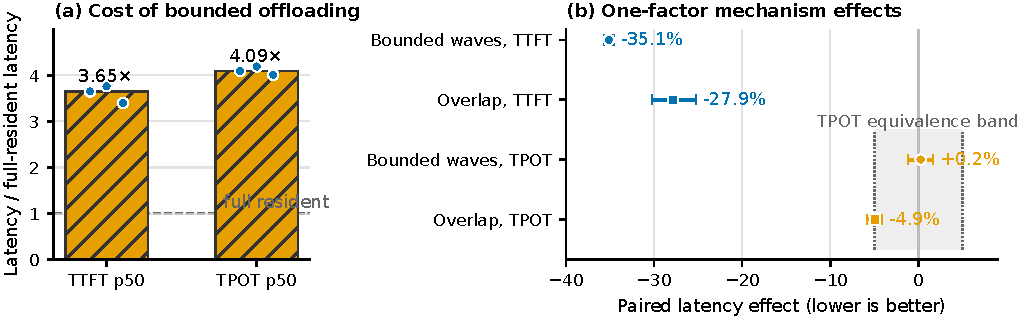
\includegraphics[width=\textwidth]{figures/baseline_mechanisms.pdf}
  \Description{Two-panel evaluation. The left panel shows LatchMoE's TTFT and
  TPOT latency ratios relative to full residency for three exact-token starts.
  The right panel is a forest plot of paired TTFT and TPOT effects for bounded
  waves and overlapped staging, including confidence intervals and the
  plus-or-minus-five-percent TPOT equivalence band.}
  \caption{Bounded offloading has an explicit full-resident cost, while its two
  prefill mechanisms reduce exposed latency. (a) Bars are medians and points
  are three fresh exact-token, counterordered starts (96 requests per arm);
  the full-resident reference is 1.0.
  Native-prefetch and legacy-offload arms are omitted because they fail the
  exact-token comparability gate. (b) Bounded waves compare multi-wave against
  full-layer staging (200 requests per unit); overlap compares prefetch depth
  one against serial depth zero (64 requests per unit). Each contrast uses
  three counterordered pairs. Points are paired log-ratio estimators; whiskers
  are 95\% CIs for TTFT and 90\% CIs for TPOT. Lower is better. All experiments
  use Qwen3-30B-A3B, one Ascend 910B2, and concurrency one.}
  \label{fig:baseline-mechanisms}
\end{figure*}

\subsection{Q1: What is the deployability trade-off?}

We run three counterordered starts of four ACLGraph arms with an explicit
512-MiB KV cache and \FormalRequestsPerBaselineUnit requests per unit:
full-resident vLLM-Ascend, its native weight-prefetch path, the legacy layered
offload path, and LatchMoE with a 14-GiB target. Full residency and LatchMoE
each pass \FormalRequestsPerBaselineArm/\FormalRequestsPerBaselineArm{} exact
requests. Native prefetch and legacy layered offload both complete
\FormalRequestsPerBaselineArm/\FormalRequestsPerBaselineArm{} requests and
capture/replay the graph, but respectively differ from the oracle on
\NativeMismatchRequests{} and \LegacyMismatchRequests{} request-token arrays
across their three starts. They remain visible feasibility cells but are
excluded from performance comparison.

Full residency is a cost anchor rather than a memory-matched offload baseline.
Its repeat-median TTFT p50 and TPOT p50 are \FullResidentTTFTMedian~ms and
\FullResidentTPOTMedian~ms/token, versus \LatchTTFTMedian~ms and
\LatchTPOTMedian~ms/token for LatchMoE. The paired TTFT effect is
+\LatchVsFullTTFTEffect\% (95\% CI [+\LatchVsFullTTFTLower\%,
+\LatchVsFullTTFTUpper\%]); the TPOT effect is +\LatchVsFullTPOTEffect\%
(95\% CI [+\LatchVsFullTPOTLower\%, +\LatchVsFullTPOTUpper\%]). In return,
the median sampled HBM peak falls from \FullResidentHBMPeak\% to
\LatchHBMPeak\%.

Table~\ref{tab:cost-anchor} makes the trade-off explicit. LatchMoE stores
13.50~GiB in the host expert store and 3.38~GiB in persistent slots, plus a
0.56~GiB prefill stage bank; the profile records 292.05~GiB of H2D traffic.
The measured 17-percentage-point HBM reduction costs 261.28\% higher TTFT p50
and 309.51\% higher TPOT p50. The result is therefore single-card
deployability with an explicit latency cost, not a universal speedup. This
trade-off matters for larger tuples: Qwen3-Next's native full-resident
end-to-end path cannot materialize on the evaluated 64-GiB device, whereas its
bounded LatchMoE qualification completes (Q6).

\begin{table}[t]
  \centering
  \small
  \caption{Same-scope full-resident cost anchor for Qwen3-30B-A3B: three fresh starts, 32 requests per arm, 512-MiB KV cache, and disabled prefix caching. HBM reclamation is the difference in median sampled peak utilization; stage wait is reported from the profile, not substituted for end-to-end latency.}
  \label{tab:cost-anchor}
  \begin{tabular}{lrr}
    \toprule
    Metric & Full resident & LatchMoE \\
    \midrule
    TTFT p50 (ms) & 179.13 & 662.22 \\
    TPOT p50 (ms/token) & 13.19 & 54.50 \\
    Output throughput (tok/s) & 52.94 & 13.23 \\
    Sampled peak HBM (\%) & 97 & 80 \\
    Host store (GiB) & 0 & 13.50 \\
    Slot HBM (GiB) & 0 & 3.38 \\
    Prefill stage HBM (GiB) & 0 & 0.56 \\
    H2D traffic (GiB) & 0 & 292.05 \\
    Prefill stage wait (ms) & 0 & 257.11 \\
    Decode ready wait (ms) & 0 & 95.05 \\
    \bottomrule
  \end{tabular}
  \vspace{2pt}
  \parbox{0.94\linewidth}{\footnotesize\emph{Derived cost:} LatchMoE reclaims 17 percentage points of sampled peak HBM, while adding +261.28\% TTFT-p50 and +309.51\% TPOT-p50 relative to full residency.}
\end{table}


\subsection{Q2: Does Graph preserve the matched slot path?}

The matched comparison changes only the execution mode from
\texttt{Slot+Eager} to \texttt{Slot+PIECEWISE}. Across ShareGPT, HumanEval,
and GSM8K, 18 fresh units form nine counterordered pairs and complete 3,384
requests. All 13,536 output token IDs match within pair, and no cross-start
oracle drift is observed. All nine Graph units configure PIECEWISE, reach the
offload staging seam, and record actual ACLGraph replay; none records an
unintended fallback of a graph-designated piece or an NPU/ACL failure. Thus
Graph replay preserves the evaluated
fixed-slot path at c1 across the three executable frozen buckets.

This four-token campaign is a semantic qualification, not a latency or task
accuracy result. LongBench remains an explicit negative cell: all 200 frozen
requests exceed the 8,192-token context/KV configuration and are neither
trimmed nor replaced. Q5 separately reports the concurrency boundary.

\begin{figure*}[!t]
  \centering
  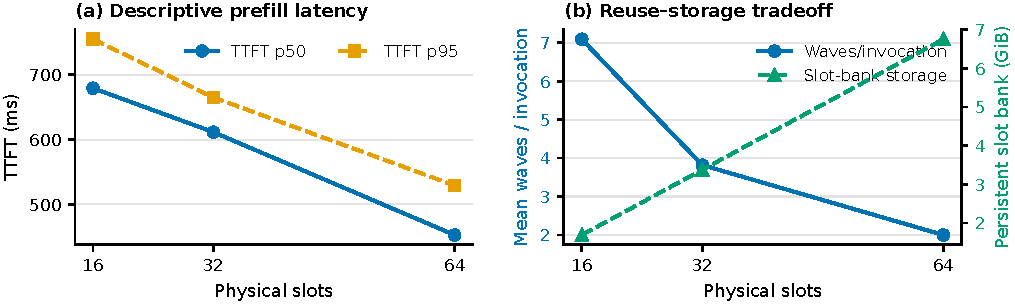
\includegraphics[width=\textwidth]{figures/capacity_sensitivity.pdf}
  \Description{Two-panel slot-capacity sensitivity. The left panel plots TTFT
  p50 and p95 at 16, 32, and 64 slots. The right panel plots mean waves per
  prefill-layer invocation and persistent slot-bank storage for those same
  capacities.}
  \caption{Online slot-capacity sensitivity for Qwen3-30B-A3B with one fresh
  start per point. All other serving controls are fixed, including a 14-GiB
  offload target, 512-MiB KV cache, \CapacityRequests{} requests, and
  concurrency one on one Ascend 910B2 with BF16 and tensor parallelism one;
  prefix caching is disabled. More slots trade persistent HBM for fewer waves;
  latency values are descriptive.}
  \label{fig:capacity}
\end{figure*}

\subsection{Q3: Do bounded waves improve full-layer staging?}

The graph-compatible full-layer arm materializes the layer working set before
compute; the multi-wave arm instead uses bounded transient banks and the
explicit eager wave executor to execute and recombine routed work. All model,
layer-selection, workload, and serving controls remain fixed, but the bounded
design necessarily changes both staging granularity and the overflow expert
path. Q3 therefore evaluates the complete bounded-wave design rather than
attributing its effect to partitioning alone. Three AB/BA/AB pairs each serve
\BoundedRequestsPerUnit{} requests. All six units complete
\BoundedTotalRequests{} requests, match all \BoundedTotalTokens{} output token
IDs and preserve the configured piecewise execution contract. Graph-designated
pieces capture and replay as required, while overflow expert waves execute
through the explicit eager path; no unit records unintended fallback or a
lifecycle error.

TTFT changes by \BoundedTTFTEffect\% with a 95\% CI of
[\BoundedTTFTLower\%, \BoundedTTFTUpper\%]. As a conventional summary, the
median across starts of TTFT p50 falls by
\BoundedRepeatMedianTTFTReduction\%, and TTFT p95 falls by
\BoundedRepeatTailTTFTReduction\%. TPOT's paired effect is
\BoundedTPOTEffect\% with a 90\% CI of
[\BoundedTPOTLower\%, \BoundedTPOTUpper\%], entirely within the
preregistered $\pm5\%$ equivalence margin. The supported result is therefore a
prefill-path TTFT reduction without a material TPOT change under this contract.

\subsection{Q4: Does overlap contribute causally?}

We next hold the wave plan, two stage banks, graph mode, slot capacity,
workload, seeds, and source digest fixed, changing only prefetch depth from
zero (serial staging) to one (overlap). Three AB/BA/AB pairs serve
\OverlapRequestsPerUnit{} requests per unit; all \OverlapTotalRequests{}
requests pass exact-token, graph, lifecycle, and release
gates. Overlap changes TTFT by \OverlapTTFTEffect\% (95\% CI
[\OverlapTTFTLower\%, \OverlapTTFTUpper\%]); the interval is entirely below
zero and passes the preregistered causal-benefit gate. TPOT changes by
\OverlapTPOTEffect\% (90\% CI [\OverlapTPOTLower\%,
\OverlapTPOTUpper\%]). Its equivalence gate does \emph{not} pass because the
lower bound extends beyond $-5\%$; we report the measured decrease rather than
calling TPOT unchanged. This one-factor experiment supports overlap's causal
contribution, while Q3 measures the complete multi-wave path.

\subsection{Q5: How robust is the slot contract?}

We sweep 16, 32, and 64 physical slots with the same model, 14-GiB target,
512-MiB KV cache, first \CapacityRequests{} manifest requests, and runtime
source digest. Each
point is one fresh start and passes exact-token, graph, capacity, lifecycle,
and release gates; latency is therefore descriptive rather than an uncertainty
claim. Figure~\ref{fig:capacity} reports the resulting TTFT, average wave count,
and persistent-slot storage. From 16 to 64 slots, TTFT p50 falls from
\SlotsSixteenTTFTMedian{} to \SlotsSixtyFourTTFTMedian{}~ms
(\CapacityTTFTMedianReduction\%), and p95 falls from
\SlotsSixteenTTFTTail{} to \SlotsSixtyFourTTFTTail{}~ms
(\CapacityTTFTTailReduction\%). Total waves fall from \SlotsSixteenWaves{} to
\SlotsSixtyFourWaves{} and H2D volume from \SlotsSixteenHtwoDGiB{} to
\SlotsSixtyFourHtwoDGiB{}~GiB, while the persistent slot bank grows from
\SlotsSixteenSlotGiB{} to \SlotsSixtyFourSlotGiB{}~GiB and sampled peak HBM
rises from \SlotsSixteenHBMPeak\% to \SlotsSixtyFourHBMPeak\%. This point
quantifies the intended
reuse--storage tradeoff; it is not a cross-workload scaling claim.

Capacity pressure also has a lifecycle dimension once requests overlap. In a
separate bounded ShareGPT stress test, concurrency two and four both trigger
real slot reuse and complete with exact outputs, monotonically increasing slot
generations, H2D-ready publication before consumption, and balanced compute
leases. This result exercises the ownership protocol beyond the c1 performance
campaigns; because it is a targeted stress test rather than an offered-load
sweep, it does not establish throughput or tail-latency scaling.
The wider \texttt{standard\_v1} qualification at concurrency eight exposes
paired exact-token exceptions in ShareGPT, HumanEval, and GSM8K. We retain that
negative result and admit none of its latency measurements; high-load
correctness and performance remain outside the supported boundary.

\subsection{Q6: Does the interface generalize across model contracts?}

\begin{table*}[t]
  \centering
  \small
  \caption{Three-model semantic and graph qualification. $L/E/S$ denotes managed MoE layers, routed experts per layer, and resident shared experts. Router/boundary counts are exact native comparisons; locks/replays are address locks and observed graph replays; overflow/H2D counts exercise the explicit eager wave path and transfer leases. Every row passes all 11 gates, including exact end-to-end tokens and zero unintended fallback of graph-designated pieces.}
  \label{tab:qualification}
  \begin{tabular}{lrrrrrrc}
    \toprule
    Model & $L/E/S$ & top-$k$ & Router & Boundary & Locks/replays & Overflow/H2D & Result \\
    \midrule
    Qwen3-30B-A3B & 48/128/0 & 8 & 192 & 192 & 48/97 & 144/239 & Pass \\
    GLM-4.7-Flash & 46/64/1 & 4 & 184 & 184 & 46/94 & 92/226 & Pass \\
    Qwen3-Next-80B-A3B & 48/512/1 & 10 & 192 & 192 & 48/97 & 144/240 & Pass \\
    \bottomrule
  \end{tabular}
\end{table*}


Table~\ref{tab:qualification} covers routed-only Qwen3-30B-A3B, shared-expert
GLM-4.7-Flash, and shared-expert Qwen3-Next-80B-A3B-Instruct. Each tuple is
checked against native routing and layer boundaries, a native end-to-end oracle
where feasible, eager-seam parity, exact output tokens, capture and replay of
graph-designated pieces, zero unintended eager fallback, explicit overflow-path
composition, decode cache churn, H2D ordering, and release. Every captured
slot/map address validates at replay,
every managed layer releases its original expert bank, and the online profiles
exercise both overflow waves and H2D leases. LatchMoE therefore preserves the
evaluated routing and combination contracts rather than merely making the
models runnable.

This is capability rather than performance generalization. Each model uses one
short request in each end-to-end mode plus a one-token overflow stress request.
Qwen3 and GLM compare native, LatchMoE-eager, and LatchMoE-graph outputs.
Qwen3-Next cannot materialize its native full-resident end-to-end path on this
device, so native semantics are checked at its router and layer boundary and
the end-to-end gate compares eager seam with Graph. We make no cross-model
latency claim.

\paragraph{Resource costs and boundaries.}

\begin{table}[t]
  \centering
  \small
  \caption{Audited resources in each model's graph-qualified LatchMoE run. Device storage sums the 32-slot bank, prefill stage banks, and resident shared-expert weights; H2D is the profiled transfer volume for that qualification workload. Original managed expert banks are released in every row.}
  \label{tab:resources}
  \begin{tabular}{lrrrr}
    \toprule
    Model & Host & Device & H2D & Replays \\
          & (GiB) & (GiB) & (GiB) & \\
    \midrule
    Qwen3-30B-A3B & 54.0 & 14.1 & 65.5 & 97 \\
    GLM-4.7-Flash & 51.8 & 26.7 & 22.3 & 94 \\
    Qwen3-Next-80B-A3B & 144.0 & 9.7 & 152.6 & 97 \\
    \bottomrule
  \end{tabular}
\end{table}


Table~\ref{tab:resources} accounts for each model's graph-qualified 32-slot
run. Host storage scales with the managed expert pool, while device storage
depends on expert shape, shared residency, and stage banks rather than total
expert count alone. Slot/stage storage is 13.5/0.56~GiB for Qwen3,
25.9/0~GiB for GLM, and 9.0/0.38~GiB for Qwen3-Next; mapping buffers are at most
0.19~MiB. Host-control time is 10.06~s, 0.073~s, and 44.85~s, respectively.
These workload-specific values are costs, not a cross-model ranking.
Qualification profiles record every original managed bank
release; formal performance and Motivation services additionally retain a
service-level release acknowledgment. The capability preflight rejects
unknown router adapters, fused shared/routed ownership, quantized expert
layouts, multi-NPU execution, and shared-expert overlap before capture. These
are retained system boundaries: the evaluation establishes a single-NPU BF16
data plane, not silent fallback or support for unqualified tuples.
